\documentclass[tikz,border=2pt]{standalone}
\usepackage{amsmath,amssymb}
\usepackage{pgfplots}
\pgfplotsset{compat=1.18}

\begin{document}
% Partial sums of the exponential series 1 + x + x^2/2! + ... : each added term extends the
% range on which the polynomial follows e^x.
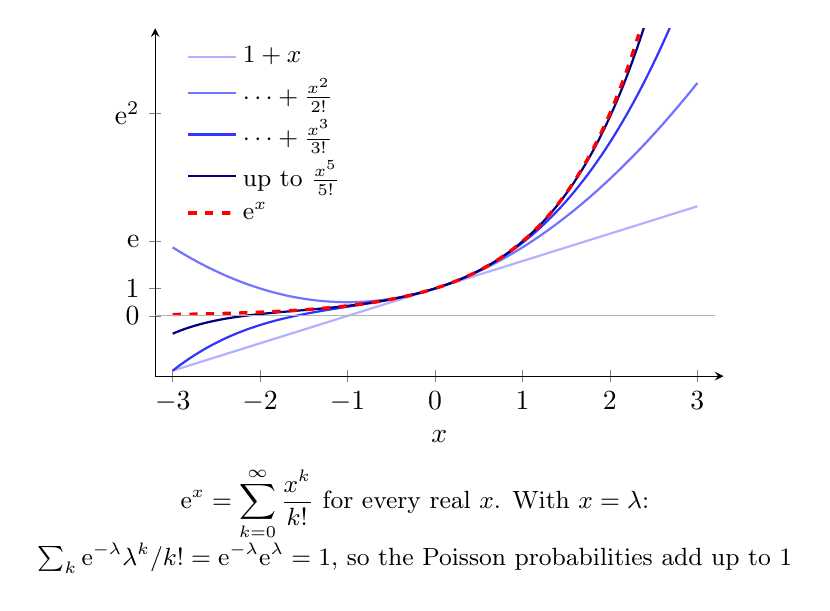
\begin{tikzpicture}
	\begin{axis}[
		axis lines=left, xmin=-3.2, xmax=3.3, ymin=-2.2, ymax=10.5,
		xtick={-3,-2,-1,0,1,2,3}, ytick={0,1,2.718,7.389}, yticklabels={$0$,$1$,$\mathrm{e}$,$\mathrm{e}^2$},
		xlabel={$x$},
		samples=140, smooth, width=8.8cm, height=6cm,
		legend style={draw=none, fill=none, font=\small, at={(0.04,0.98)}, anchor=north west}, legend cell align=left
		]
		\addplot[blue!30, thick, domain=-3:3] {1+x};
		\addlegendentry{$1+x$}
		\addplot[blue!55, thick, domain=-3:3] {1+x+x^2/2};
		\addlegendentry{$\cdots+\tfrac{x^2}{2!}$}
		\addplot[blue!80, thick, domain=-3:3] {1+x+x^2/2+x^3/6};
		\addlegendentry{$\cdots+\tfrac{x^3}{3!}$}
		\addplot[blue!50!black, thick, domain=-3:2.75] {1+x+x^2/2+x^3/6+x^4/24+x^5/120};
		\addlegendentry{up to $\tfrac{x^5}{5!}$}
		\addplot[red, very thick, dashed, domain=-3:2.33] {exp(x)};
		\addlegendentry{$\mathrm{e}^x$}
		\draw[gray!60] (axis cs:-3.2,0) -- (axis cs:3.2,0);
	\end{axis}
	\node[anchor=north, font=\small, align=flush center, text width=9.6cm] at ([yshift=-2pt]current axis.outer south) {$\mathrm{e}^x=\displaystyle\sum_{k=0}^{\infty}\frac{x^k}{k!}$ for every real $x$. With $x=\lambda$: $\sum_{k}\mathrm{e}^{-\lambda}\lambda^k/k!=\mathrm{e}^{-\lambda}\mathrm{e}^{\lambda}=1$, so the Poisson probabilities add up to $1$};
\end{tikzpicture}
\end{document}
